
\begin{margintable}
\begin{tabularx}{\textwidth}{ |X|X|X| }
  \hline
   & \bf{POP} & \bf{merged T/P - ERS-1 }  \\
  \hline
  dx & $7km-11km$  & $1/3^{\circ}$ ($\approx 40 km$ after filtering)  \\
  \hline
  dt & $1d$  & $7d$  \\
  \hline
  $\log_{10}2$ filter cutoff & \na  & $2^{\circ} $ by $ 2^{\circ} $  \\
  \hline
  z-levels & 42  & 1  \\
  \hline
  variables & SSH, S, T, u/v/w, tracers etc & \SSH~ \\
  \hline
	pot. interpolation artifacts & \na  & yes  \\
  \hline
	reality & no  & yes  \\
  \hline
\end{tabularx}
%\caption[model vs satellite][5pt]{model vs satellite data}
\label{table:modVSsat}
\end{margintable}

\newthought{The } latest \AVI~\SSH~data from satellites features impressive accuracy, constancy and resolutions in both space and time. This is achieved
by collecting all of the data from all of the altimeter-equipped satellites available at any given moment for any given coordinate. This conglomerate of highly
inhomogeneous data is then subjected to state-of-the-art interpolation methods to produce a spatially and temporally coherent product. One satellite alone is
not sufficient to adequately resolve mesoscale variability globally.
\begin{marginfigure}
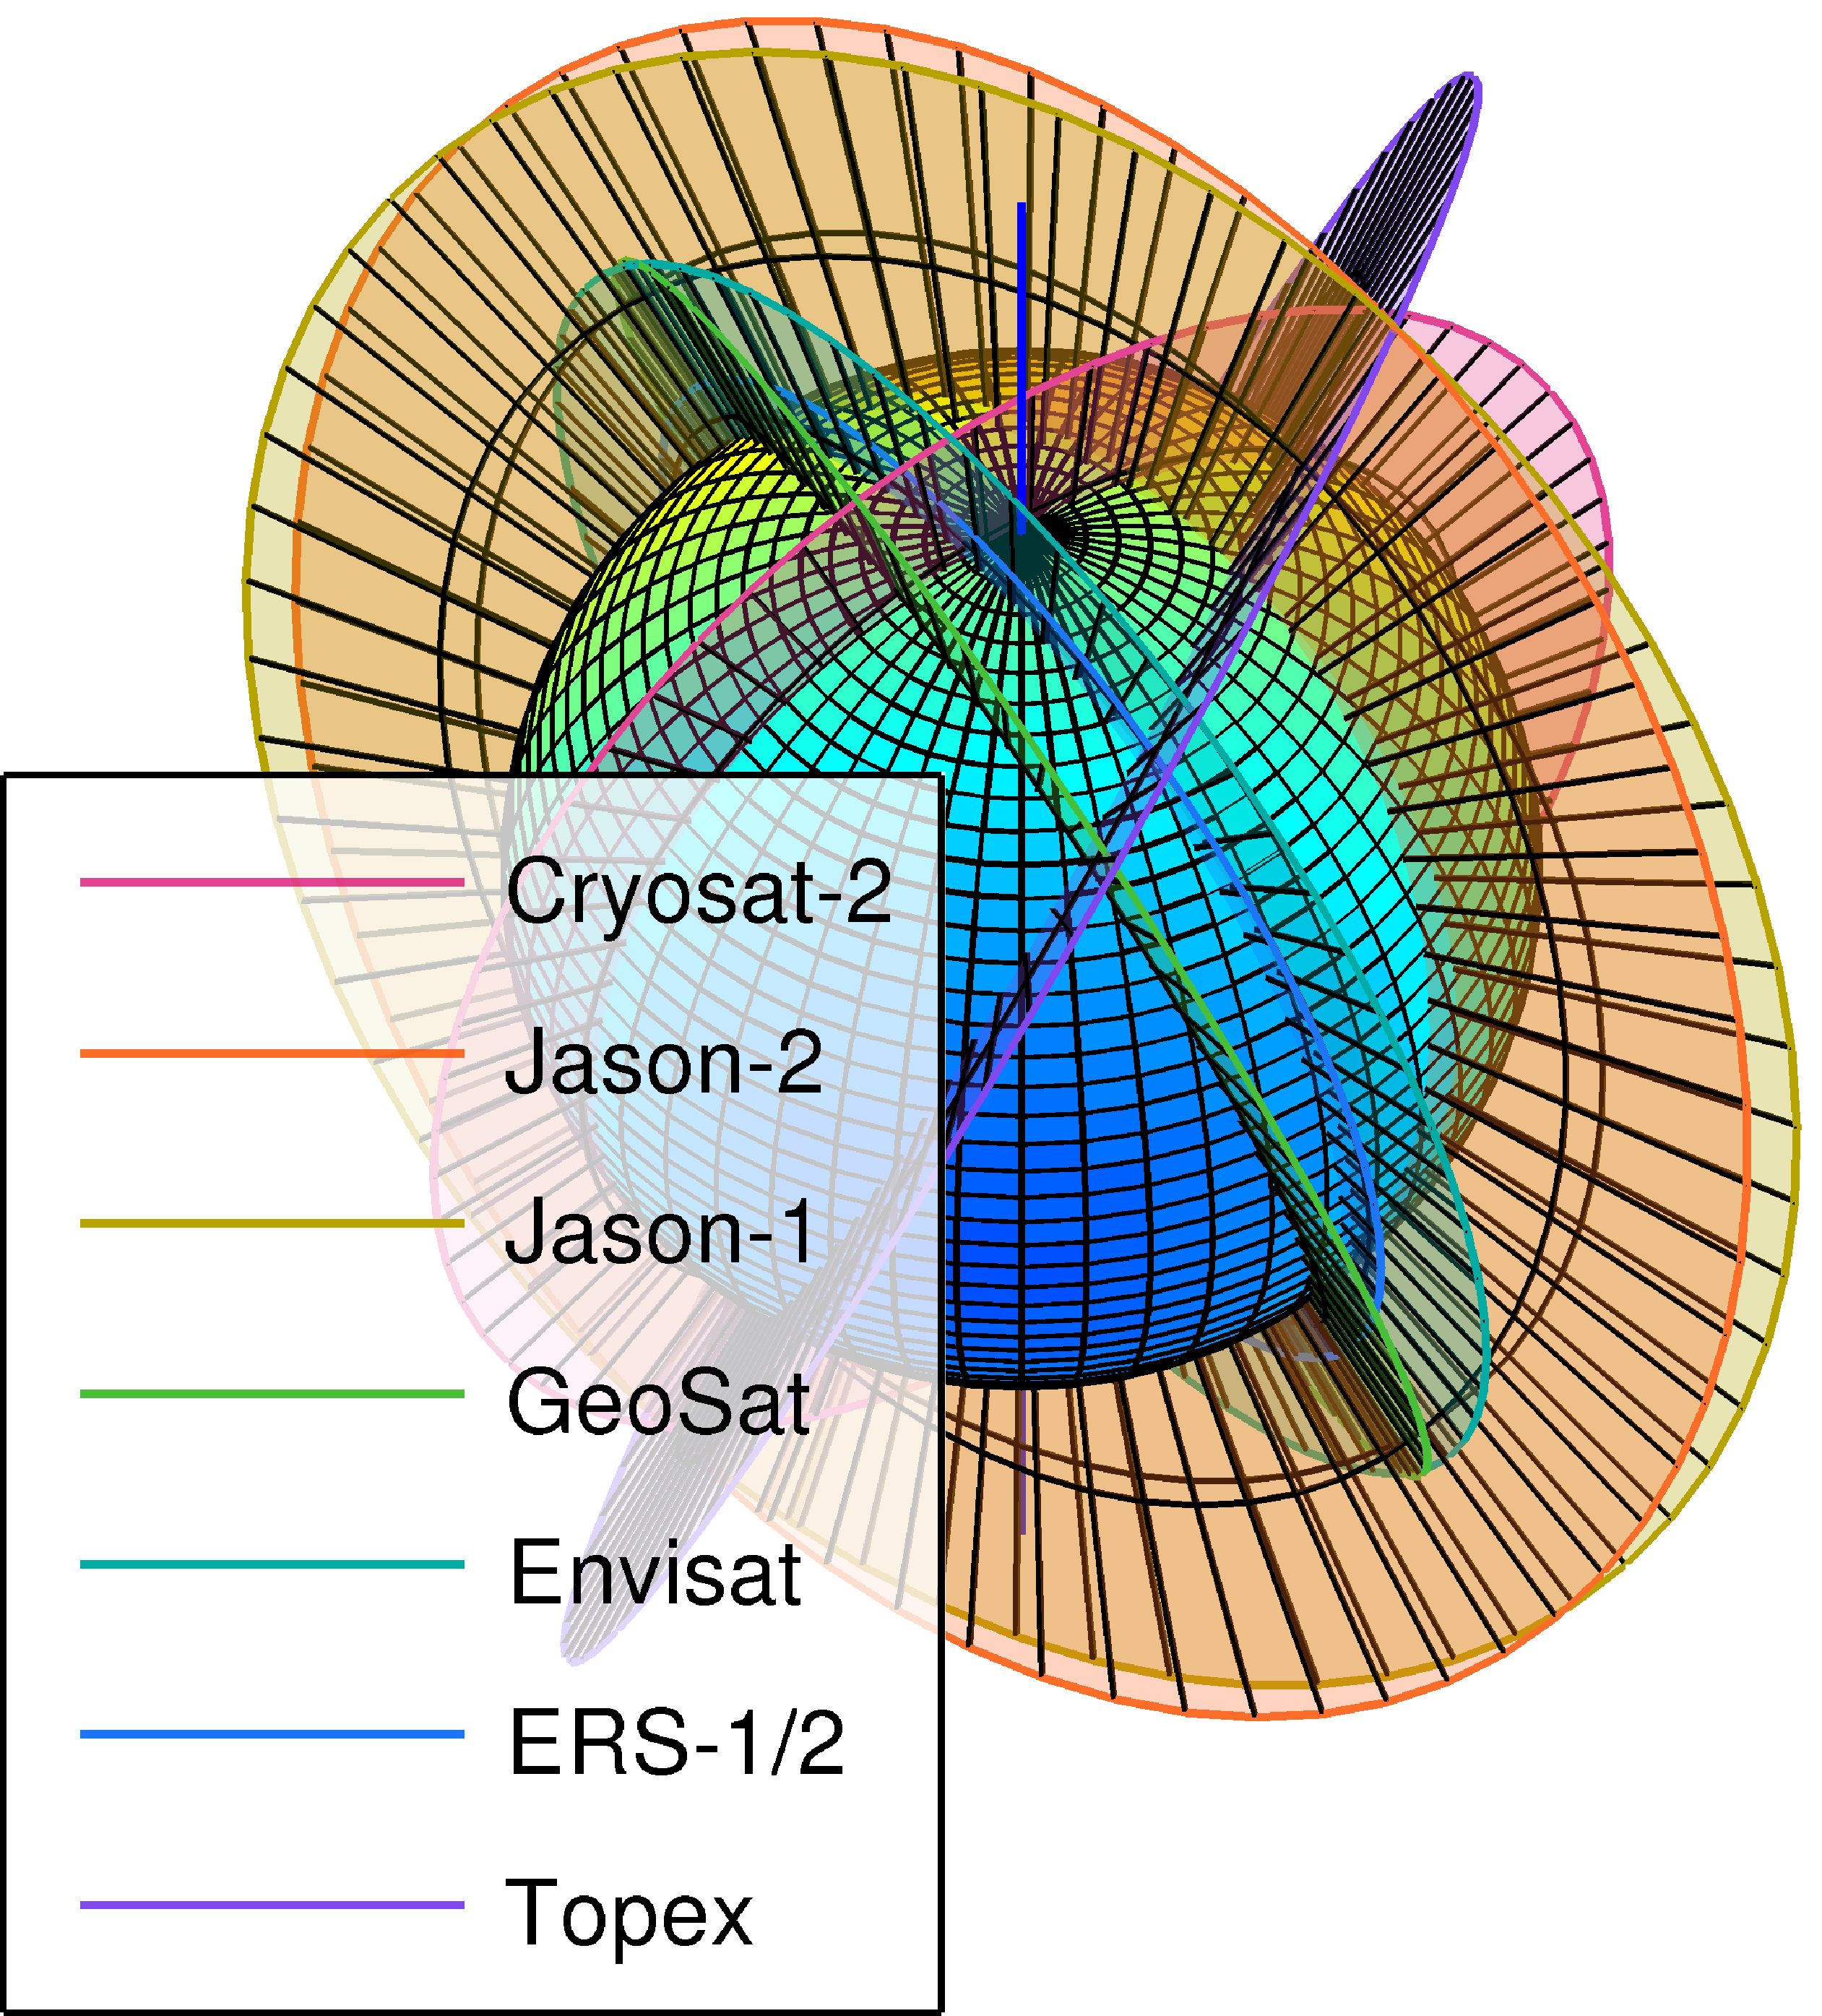
\includegraphics[]{orbits3.pdf}
%\caption{Orbits for Aviso-relevant satellites.}
\end{marginfigure}
\Eg the Topex/Poseidon satellite had a ground repeat track orbit of 10 days and circled the earth in 112 minutes or $\approx 13$ times a day with a swath width of 5 km. Hence it drew $\sim 26$ 5-km-wide stripes onto the globe every day.
The orbit's precession is such that this pattern is then repeated after 10 days, which means that at the equator only  $10 \times 26 \times 5 = \SI{1300}{\km}$ of the $2\pi \times 6371=\SI{40000}{\km}$ get covered, \ie $3.25\%$. At every $\SI{10}{\day}$ time-step, on average, effectively $(40000-1300)/26 = \SI{1490}{\km}$ are left blank in-between swaths on the equator. This is why, no matter how fine the resolution within the swath at one moment in time may be, the spatial resolution is so coarse.
The merged ERS-1/Topex-data as used by \citet{Chelton2011} has a time step of 7 days. Assuming eddy drift speeds of $u_e= \order{-1}\si{\m/\s}$ implies a distance traveled per time step of $L_{\delta t}\approx \SI{60}{\km}$. \citeauthor{Chelton2011} estimate their effective spatial resolution as $\delta x \approx \SI{40}{\km}$. Eddies of smaller scale are not resolved.
\begin{figure}
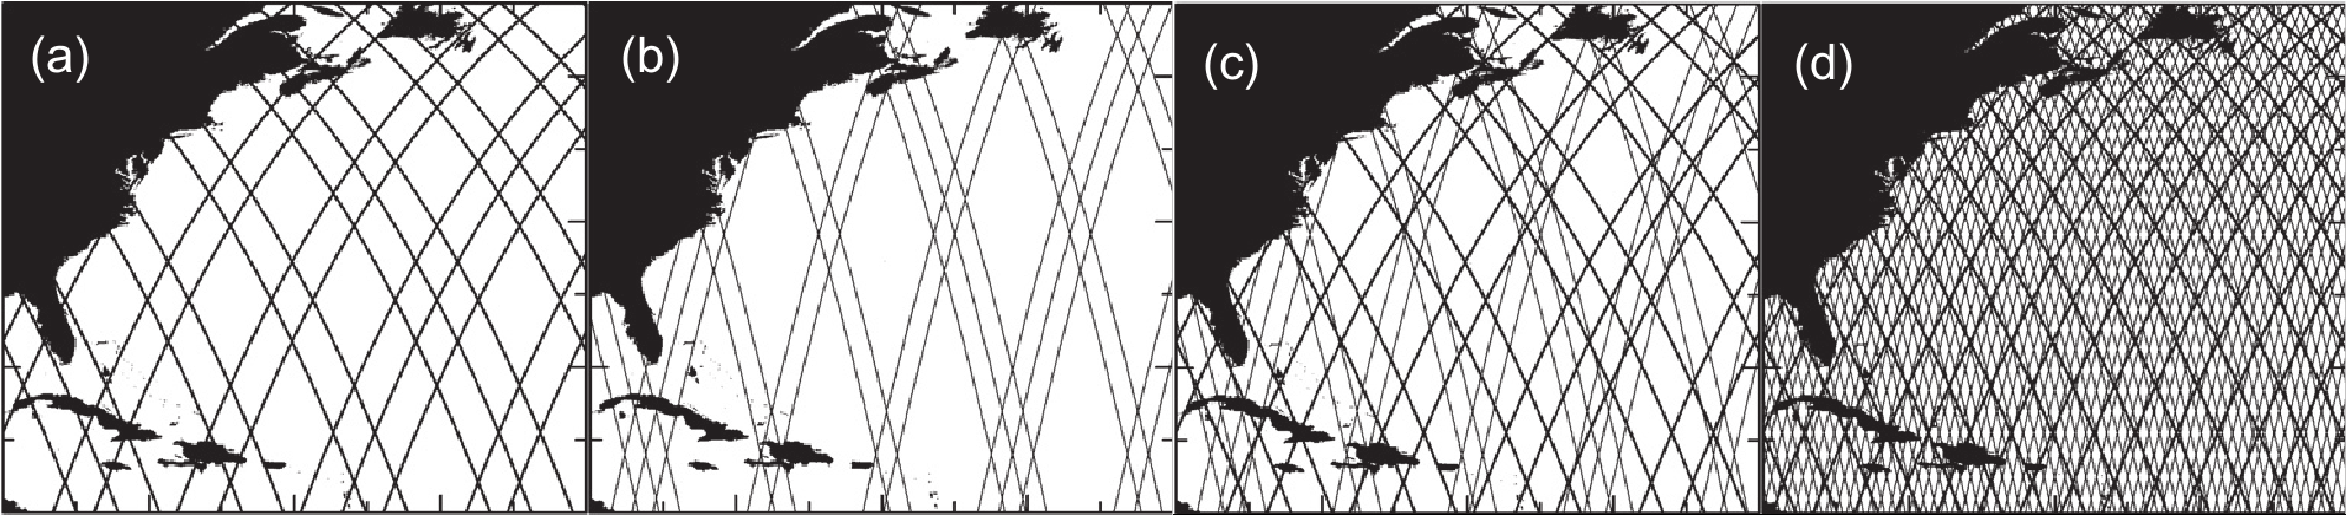
\includegraphics[]{tracks.pdf}
\caption{{The ground track patterns for the 10-day repeat orbit of T/P and its successors Jason-1 and Jason-2 (thick lines) and the 35-day repeat orbit of ERS-1 and its successors ERS-2 and Envisat (thin lines). (a) The ground tracks of the 10-day orbit during a representative 7-day period; (b) The ground tracks of the 35-day orbit during the same representative 7-day period; (c) The combined ground tracks of the 10-day orbit and the 35-day orbit during the 7-day period; and (d) The combined ground tracks of the 10-day orbit and the 35-day orbit during the full 35 days of the 35-day orbit. (sic)} \citep{Chelton2011}}
\end{figure}

\newthought{Tracking}~a single eddy from one time-step to the next is complicated by the sheer abundance of eddies at any given point in time and the fact that eddy activity is usually concentrated into regions of strong geostrophic turbulence.
The ambiguities in matching the eddies from the old time-step to those of the new one might cause aliasing effects in the final statistics.
\begin{figure}
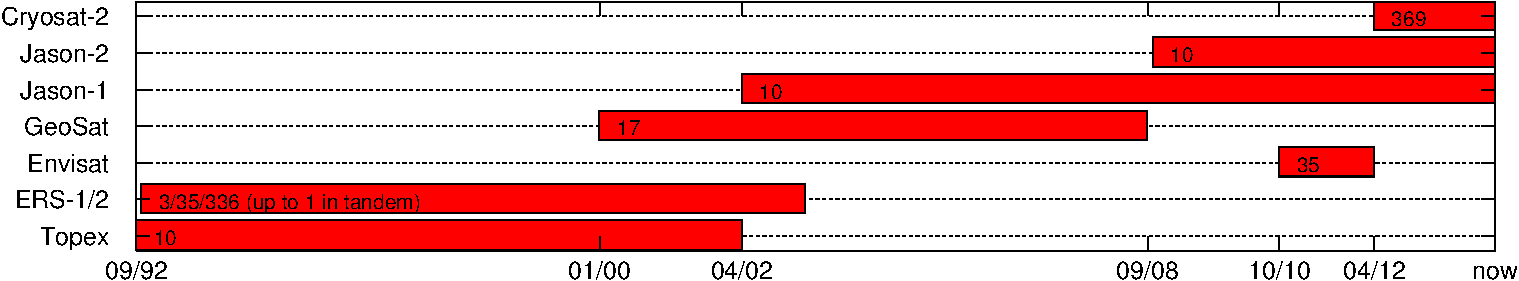
\includegraphics[]{sats.pdf}
\caption{Length of mission. Numbers are orbit-period in days.}
\label{fig:lengthOfMission}
\end{figure}

\newthought{The }  translational speeds \footnote{$\order{1}$km/day} of eddies are not really the problem here, as they usually drift slow enough to not cover more
than 1 grid node per 7 day time step. The issue are those areas where eddies are born, die and merge. According to \citet{Smith2009}, instabilities within the ACC
grow at rates of up to $1/(2 \mathrm{days})$, which means that at one time-step up to 3 eddies have emerged and equally many died for every eddy identified within
such region. The ground-repeat-frequency of a satellite can of course not be set arbitrarily. Especially when the satellite is desired to cover as far north and
south as possible, whilst still being subjected to just the right torque from the earth's variable gravitational field to precess at preferably a
sun-synchronous frequency \ie $360^{\circ}/year$ \citep{goldreich1965inclination}. Neither can the
satellite's altitude be chosen arbitrarily. If too low the oblateness of the earth creates too much eccentricity in the orbit that can no longer be
\textit{frozen} \footnote{minimizing undulating signals in altitude by choosing the right initial values \citep{goldreich1965inclination}}. Another problem could be potential inhomogeneity in
the merged data in time dimension, since data of old and current missions are lumped together into one product. This is why \citet{Chelton2011} opted against
the finest resolution available and instead went for a product that had the most satellites merged in unison for the longest period of time.

\newthought{The } surface velocities inferred from altimetry are the geostrophic components only, which should suffice to \eg determine the non-linearity and kinetic energy of an eddy for almost all regions, but less so for \eg the western boundary currents.
%%####################################################################
%%####################################################################
\begin{marginfigure}
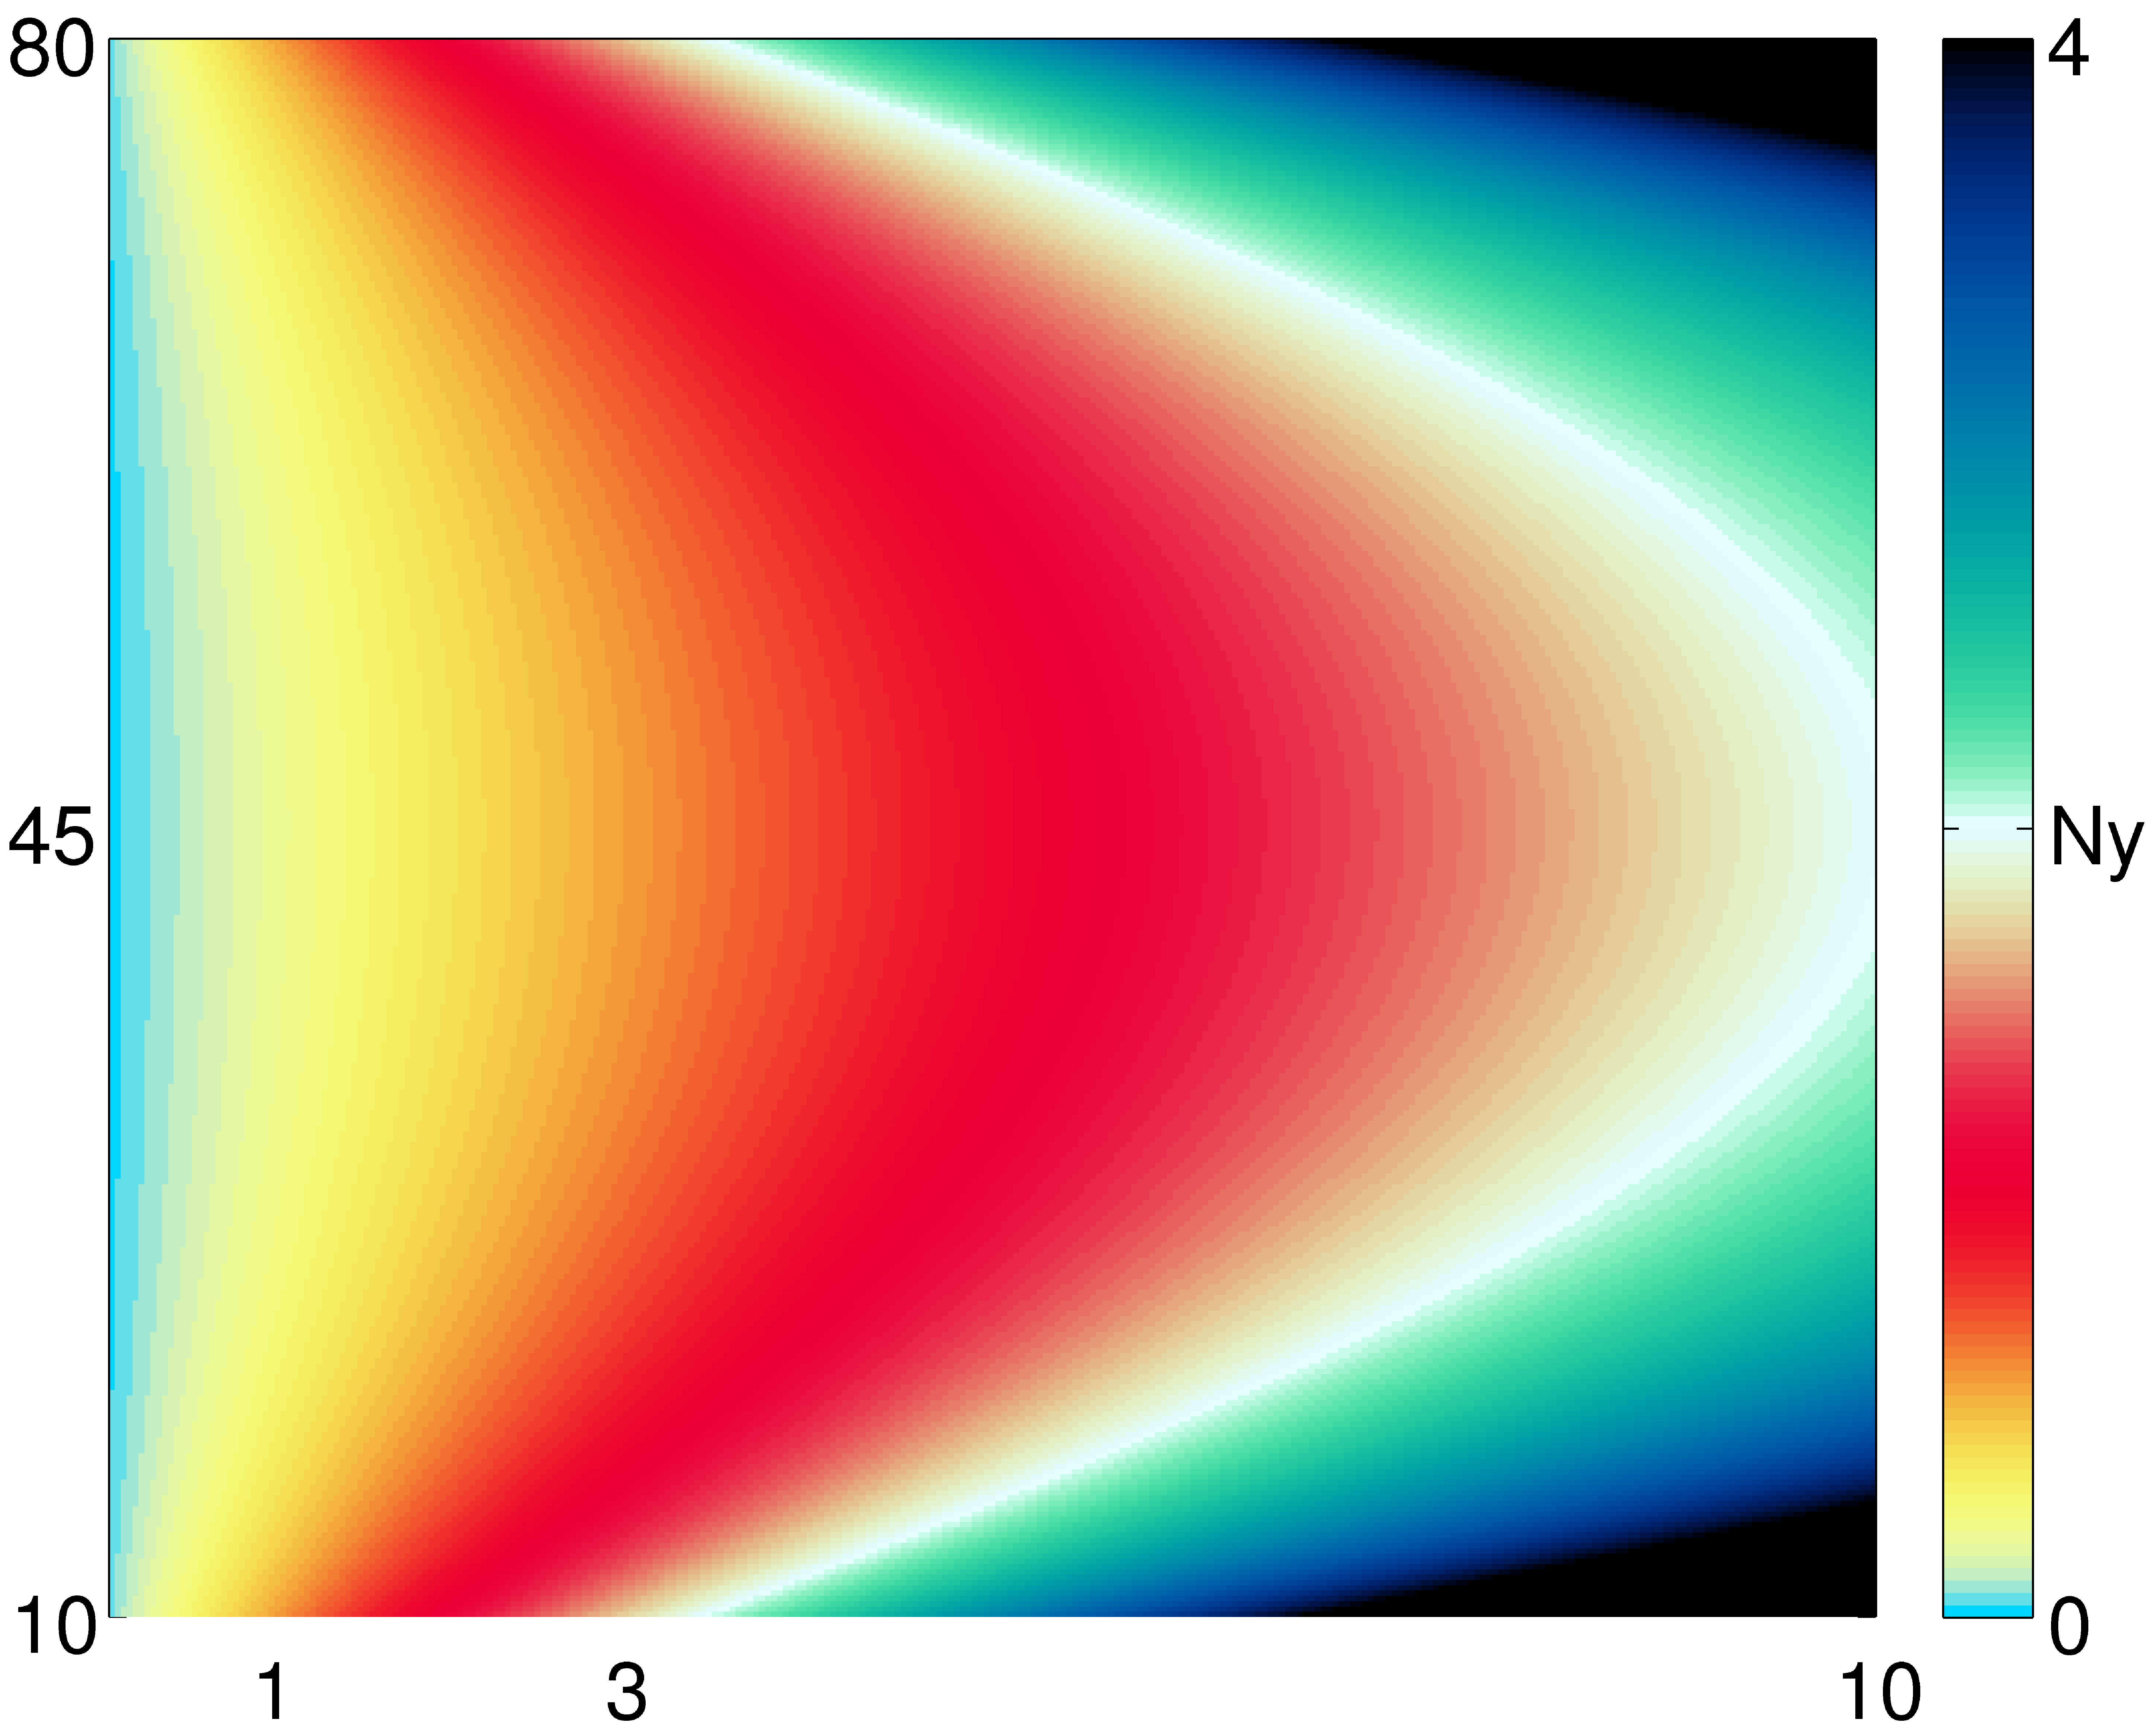
\includegraphics[]{latovermu}
\caption{$\xi(\phi,\mu)$. $\mathrm{Ny}\equiv 2$ \ie the Nyquist frequency.}
\label{fig:latovermu}
\end{marginfigure}

\begin{infobox}[Horizontal Resolution]
\label{box:horRes}
Assume $\Bu=1$, so that $L=NH/f$ and $NH=a/10d$ (corresponds to $L(\phi=30^{\circ})=100$km), a model resolution of $1^{\circ}/\mu$ and that the eddy diameter was twice the Rossby radius. Then, how many grid notes $\xi$ fit into one eddy as a function of latitude?
%%....................................................................
\begin{align}
	\xi \frac{a}{\mu} \frac{\cos \phi}{2 \pi}
	&=
	\frac{2NH }{f} = \frac{2NH 1d}{4 \pi  \sin(\phi)}\notag\\
	\xi
	&=
	 \frac{ 2\mu }{10  \sin(2\phi)}\notag\\
\end{align}
In this flat-bottom, constant $\rho_z$, Mercator-gridded model the worst eddy-resolution is interestingly at mid-latitude (see \cref{fig:latovermu}).
\end{infobox}

\newthought{The}~finer resolution of the \POP~data in space and time should certainly yield more precise results.
It must be kept in mind though that by using the model data, what one analyses is of course just that - a \emph{model}. Baroclinic geostrophic space/time scales depend crucially on \eg the vertical density structure (see \cref{sec:hist_cush}, \citet{Rhines1979}), which is resolved only poorly in the model. A useful comparison among satellite/model results should hence be tricky.   
